% Seminar Information Retrieval Philipp Schalcher
% Betreuer: Ruxandra Domenig
% Thema: Evaluierung der Retrieval-Leistung einer Search Engine am Beispiel einer privaten MP3-Sammlung

\documentclass[12pt,a4paper,ngerman]{report}
\setlength{\parindent}{0pt}
\usepackage[ngerman]{babel}
\usepackage[utf8]{inputenc}
\usepackage{a4wide}
\usepackage{graphicx}
\usepackage{url}
\usepackage[final]{listings}
\usepackage{color}
\usepackage{amsmath}
\author{Philipp Schalcher}
\title{Evaluierung der Retrieval-Leistung einer Search Engine am Beispiel einer privaten MP3-Sammlung}
\date{\today}

\begin{document}
%\maketitle
\begin{titlepage}
\begin{center}

\includegraphics[width=0.25\textwidth]{img/zhaw.png}\\[0.5cm]
\textsc{\Large Zürcher Hochschule für Angewandte Wissenschaften}\\[1.0cm]
\textsc{\Large Seminar Information Retrieval}\\[1.5cm]

% Title
\hrulefill \\[0.5cm]
{\huge \bfseries Evaluierung der Retrieval-Leistung einer Search Engine am Beispiel einer privaten MP3-Sammlung}\\[0.4cm]
\hrulefill \\[0.5cm]
%Author und Betreuer
\begin{minipage}{0.4\textwidth}
\begin{flushleft}
\emph{Author:}\\
Philipp \textsc{Schalcher}
\end{flushleft}
\end{minipage}
\begin{minipage}{0.4\textwidth}
\begin{flushright}
\emph{Betreuer:}\\
Ruxandra \textsc{Domenig}
\end{flushright}
\end{minipage}

\vfill

%Datum
{\large \today}

\end{center}
\end{titlepage}
\chapter*{Danksagung}
\tableofcontents
\begin{abstract}

\end{abstract}
\chapter{Einleitung}
In der heutigen Zeit wird der Mensch von einer Fülle an Informationen überflutet. Würde er nicht gewisse Eindrücke selber filtern, könnte das zu einem Kollaps führen. Der Mensch hat das Glück, solche Dinge von der Natur eingebaut zu haben. Im Gegensatz zum Menschen besitzen Informationssysteme keine integrierten Filter. Das beste Beispiel hierfür ist Google. Es gibt eine riesige Menge an Daten, die der Suchmaschine ihr Wissen verleiht.
\\
\\
Lucene ist eine Bibliothek, welche in verschiedene Projekte eingebaut werden kann, um so eine mächtige Suchmaschine auf Basis von Indexen zu bekommen. Lucene enthält alle relevanten Funktionen, die benötigt werden, um Informationen zu durchsuchen. Hier liegt die Herausforderung, eine Suchmaschine für ID3-Tags von MP3-Dateien zu bauen, da Lucene hauptsächlich für Textdateien (PDF,TXT,DOCX,eBooks,usw.) genutzt wird. Für MP3-Dateien stehen andere Probleme an (Wie extrahiere ich die ID3-Tags aus einer MP3-Datei). 
\\
\\
Diese Arbeit soll die Information Retrieval Leistung der Suchengine Lucene analysieren. Darin enthalten sind eine Programmierung einer kleinen Suchmaschine, die MP3-Dateien innerhalb eines Ordners indexiert und danach durchsucht. Dabei beschränke ich mich in der praktischen Arbeit auf das indexieren der ID3-Tags. Diese Arbeit soll nicht als Anleitung zur Erstellung einer Suchmaschine dienen!
\\
\\
Da Lucene natürlich auch den Inhalt einer Datei analysiert, muss diese Arbeit ein bisschen angepasst werden. Da MP3-Dateien keinen Text als Inhalt haben, möchte ich daher nur theoretisch aufzeigen, wie anhand von Teilen eines Liedes das entsprechende Lied gesucht werden kann. Dies zu programmieren sprengt den Rahmen der Arbeit, somit werde ich am Beispiel von Shazam nur eine theoretische Lösung aufzeigen.
\chapter{Hauptteil}
\section*{Lucene}
Was ist Lucene? Dies ist die erste Frage, die ich mir zu Beginn der Arbeit gestellt habe. Da mir das Produkt gänzlich unbekannt war, galt es zuerst Informationen zu sammeln.\\
\\
Apache Lucene eine Suchengine, die sich auf Text und eine hohe Performance spezialisiert hat. Dabei ist die Engine mittlerweile in verschiedene Sprachen übersetzt worden. Der Apache Lucene Core ist der Hauptteil der Software und ist in Java geschrieben. Das beste an Lucene ist wohl, dass es gratis zur Verfügung steht. Somit kann jeder Entwickler eine mächtige Suchmaschine in seine Programme einbauen. \\
\\
Bei einer Suchmaschine liegen die Stärken im Resultat welches geliefert wird. Lucene bietet auch hier wieder einige Funktionen, die das Endergebnis schnell und korrekt ergeben sollen. Dazu gehören:
\begin{itemize}
	\item Ranked Searching - Die besten Resultate werden als Erste zurückgegeben.
	\item Verschiedene Query-Typen
	\item Feldsuche (Hier Titel, Album, Künstler, Jahr, Songtext).
	\item Mehrfache Indexe durchsuchen mit zusammengefasstem Ergebnis.
	\item Schnell
	\item Speichereffizient
	\item Tippfehler-tolerant
\end{itemize}
Mit diesen und weiteren Gimmicks wird Lucene auf der Webseite \url{lucene.apache.org/core/} angepriesen. Für meine Arbeit habe ich die Bibliothek in der Version 3.6.2 verwendet, da meine Quelle ebenfalls mit einer 3er-Version gearbeitet hat.
\section*{Information Retrieval}
\begin{quote}
The IR Problem: The primary goal of an IR system is to retrieve all the documents that are relevant to a user query while retrieving as few non-relevant documents as possible. - Buch: Modern Information Retrieval
\end{quote}
Dieses Zitat bezeichnet sehr gut um was es bei Information Retrieval geht. Die Menschheit speichert seit 5000 Jahren Informationen in verschiedenen Systemen, um danach über Indexe oder andere Suchmechanismen an wichtige Informationen zu kommen. Im einfachsten Fall möchte ein User nach einer Suche einen Link zu einer Webseite von einer Organisation, Firma oder sonstigen Quelle. Information Retrieval alleine dreht sich nicht nur um Suchmaschinen. Die Definition aus dem Buch Modern Information Retrieval lautet wie folgt:
\begin{quote}
Information retrieval deals with the representation, storage, organization of, and access to information items such as documents, Web pages, online catalogs, structured and semi-structured records, multimedia objects. The representation and organization of the information items should be such as to provide the users with easy access to information of their interest. - Buch: Modern Information Retrieval
\end{quote}
Zu Beginn war Information Retrieval nur eine Kategorie, die für Bibliothekare und Informationsexperten interessant war. Dieser Umstand änderte sich aber schlagartig, als das Internet aufkam. Informationen waren nun zugänglich und konnten von fast jedem Menschen abgerufen werden. Mit dem Internet wurde es wichtiger, gute Ergebnisse beim Suchen nach Informationen zu bekommen. Information Retrieval hatte die breite Masse erreicht.\\
\\
Ein Grundproblem bei IR-Systemen ist, welche Informationen für die gewünschte Suche überhaupt relevant sind. Wie soll die Software entscheiden, welche Informationen am besten auf die Anforderungen des Benutzers zutreffen? Dabei gibt es verschiedene Möglichkeiten. Ein Beispiel ist das sogenannte Ranking. Dabei wird einem Dokument, welches häufiger erscheint, ein höheres Ranking gegeben. Somit weiss die Suchmaschine, dass es wahrscheinlicher ist, dass in diesem Dokument gesuchte Informationen zu finden sind, die mit den Anforderungen übereinstimmen.\\
Eine weitere Möglichkeit besteht in der örtlichen Ablage von Informationen. So können die \textquotedblleft am nächsten liegenden\textquotedblright Informationen auch die richtigen sein. Suche ich zum Beispiel in Google nach einem Detailhändler, möchte ich natürlich die Händler im Ergebnis erhalten, die am nächsten zu mir liegen.\\
Als Drittes ist die Grösse eines Dokumentes ebenfalls eine Variable. So können kleine Dokumente bevorzugt werden, da sie schnell heruntergeladen und veranschaulicht werden können.
\newpage
Information Retrieval Systeme müssen komplexe Anforderungen erfüllen. Mit den oben genannten drei Beispielen für Ergebnissen, folgt der Schluss, dass IR-Systeme nie die eine perfekte Lösung anbieten können. Die Anfragen sind zu komplex um alle möglichen Varianten in eine Suchmaschine zu integrieren.\\
\\
Lucene ist genau solch ein IR-System. Dieses System soll nun analysiert werden. Darunter fällt die Analyse der verschiedenen Analyzer. Konkret handelt es sich um den Standard Analyzer, den Whitespace Analyzer, den Stop Analyzer und den Simple Analyzer. Hier möchte ich mich darauf konzentrieren, wie genau die Informationen in den Index gespeichert werden. Ein ebenfalls wichtiger Faktor ist die Zeit. Einerseits die Dauer der Indexerstellung und danach die Dauer der Suche mit den verschiedenen Einstellungen. Als Letztes möchte ich mich um die Analyse des Ergebnisses kümmern, wobei ich eine Testmenge an MP3 benutze um damit die tatsächlichen Suchergebnisse mit der erwarteten Menge zu vergleichen.
\section*{Lucene Search Engine}
Das entwickelte Programm hat den Namen \textquotedblleft Lucene Search Engine\textquotedblright und wurde in Java entwickelt. Im Programm kann unter dem Punkt \textquotedblleft Pfad\textquotedblright der Ablageort der MP3-Dateien angegeben werden. Mit dem Button Index wird dann in diesem Pfad ein Ordner Index erstellt, in welchem der Lucene-Index erstellt wird. Dabei durchsucht das Programm alle MP3-Dateien im angegeben Pfad, auch in Unterordnern. Aus diesen Dateien werden dann die Informationen Titel, Album, Künstler, Jahr, Songtext, Pfad und Dateiname extrahiert und in den Index geschrieben. Gesucht wird dann in den Feldern Titel, Album, Künstler, Jahr, Songtext und Dateiname. Als Ergebnis wird der Pfad zur entsprechenden Dateien ausgegeben.
\newpage
\subsection*{Das GUI}
In diesem Abschnitt möchte ich ganz kurz die grafische Benutzeroberfläche erläutern. Ich gehe nicht weiter auf die Programmierung ein, da dies nur ein kleiner, eher unwichtiger Teil der Search Engine ist.
\begin{figure}[h!]
\centering
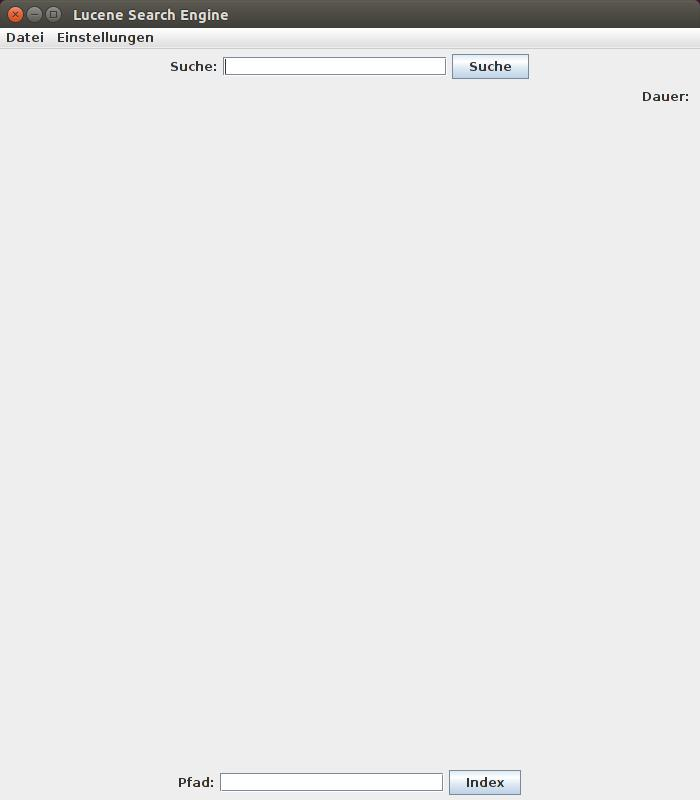
\includegraphics[width=10cm]{img/Lucene_Search_Engine_1.jpg}
\caption{GUI des Programmes\protect\footnotemark}
\end{figure}
\footnotetext{Quelle: Screenshot}
Zuerst betrachten wir die Menüleiste. Unter dem Punkt Datei ist nicht weiteres zu finden als ein Punkt \textquotedblleft Schliessen\textquotedblright der das Programm beendet. Interessanter ist da der Punkt Einstellungen. Öffnet man diesen, erhält man eine Auswahl der 4 erwähnten Analyzer. Je nach Auswahl wird der Index auf andere Weise erstellt und die Suche durchgeführt. Es kann jeweils nur ein Analyzer ausgewählt werden. Falls man ihn ändert sollte man auch den Index neu erstellen.
\subsubsection*{Indexieren}
Am unteren Rand der Applikation befindet sich das Feld Pfad. Dort wird der Pfad zu den abgelegten Dateien eingefügt. Dies funktioniert für Linux wie für Windows und Mac. Sobald dies erledigt wurde, kann mit dem Knopf die Indexierung gestartet werden. Als Analyzer wird die Auswahl aus den Einstellungen genommen. Der Index wird im gleichen Pfad erstellt und in einem Unterordner mit dem Namen \textquotedblleft Index\textquotedblright abgelegt. Dies geschieht automatisch und kann nicht geändert werden. Sobald die Indexierung beendet ist, wird auf der rechten Seite die Dauer in Millisekunden angezeigt. Je mehr MP3-Dateien indexiert werden müssen, desto länger dauert der Vorgang.
\begin{figure}[h!]
\centering

\includegraphics[width=10cm]{img/Pfadangabe.png}
\caption{Beispiel eines angegebenen Pfades in Ubuntu\protect\footnotemark}
\end{figure}
\footnotetext{Quelle: Screenshot}
Nach der Indexierung ist die Suchmaschine bereit und kann verwendet werden. Das praktische an dieser Lösung liegt darin, dass die MP3-Dateien zum Beispiel auch auf einem externen Speichermedium liegen können und der Index auf diesem Medium erstellt werden kann (gilt natürlich nicht für CD/DVDs). So kann theoretisch für jeden Ablageort eine eigener Index erstellt werden. Genaueres zur Indexierung und wie sie gelöst wurde ist im Abschnit \textquotedblleft Der Indexer\textquotedblright zu lesen.
\subsubsection*{Suchen}
Als Erstes muss gesagt werden, dass für die Suche das Pfadfeld weiterhin den Eintrag enthalten muss. Dies ist wichtig, da sonst die Engine nicht weiss, wo sich der Index befindet. Am oberen Rand befindet sich das Suchfeld. Der Benutzer kann hier seine Suchbegriffe eingeben, welche danach im Index gesucht werden. Wieder aktiviert man mit einem Klick auf Suche die Aktion. Sobald die Engine die Ergebnisse bekommen hat, wird die Dauer der Suche am rechten Rand angezeigt. Unterhalb des Suchfeldes wird eine Tabelle ausgegeben, welche die gefundenen Resultate beinhaltet.
\begin{figure}[h!]
\centering

\includegraphics[width=10cm]{img/suche.png}
\caption{Beispiel eines eingegebenen Suchbegriffes\protect\footnotemark}
\end{figure}
\footnotetext{Quelle: Screenshot}
Lucene bietet integrierte Funktionen, um die Suche besser auf seine Wünsche anzupassen. Hier ist eine Liste, wie man mit der Suchmaschine detaillierter suchen kann:
\begin{itemize}
	\item Eingabe: song1\\Sucht in den indexierten Feldern nach diesem Begriff
	\item Eingabe: song1 song2\\Sucht in den indexierten Feldern nach den beiden Begriffen. Gibt Resultate aus, welche Begriff 1 oder Begriff 2 oder beide beinhalten.
	\item Eingabe +song1 +song2\\Sucht in den indexierten Feldern nach den beiden Begriffen. Gibt Resultate aus, welche beide Begriffe beinhalten.
	\item Titel:song1\\Sucht in dem indexierten Feld Titel nach dem Begriff.
	\item Titel:song1 -Album:album1\\Sucht in den indexierten Feldern nach dem Begriff. Gibt als Resultat die Dateien zurück, welche den Titel besitzen aber nicht zum Album gehören.
	\item (song1 OR song2) AND album1\\Sucht in den indexierten Feldern nach den Begriffen. Gibt als Resultat die Dateien zurück welche song1 oder song2 im besitzen und in album1 zu finden sind.
	\item \textquotedblleft song1\textquotedblright \\Sucht in den indexierten Feldern nach exakt diesem Wort oder Text.
	\item song1*\\Sucht in den indexierten Feldern nach Werten, die mit song1 beginnen.
	\item song1$\sim$\\Sucht in den indexierten Feldern nach Werten, die ähnlich wie song1 sind.
\end{itemize}
\begin{figure}[h!]
\centering
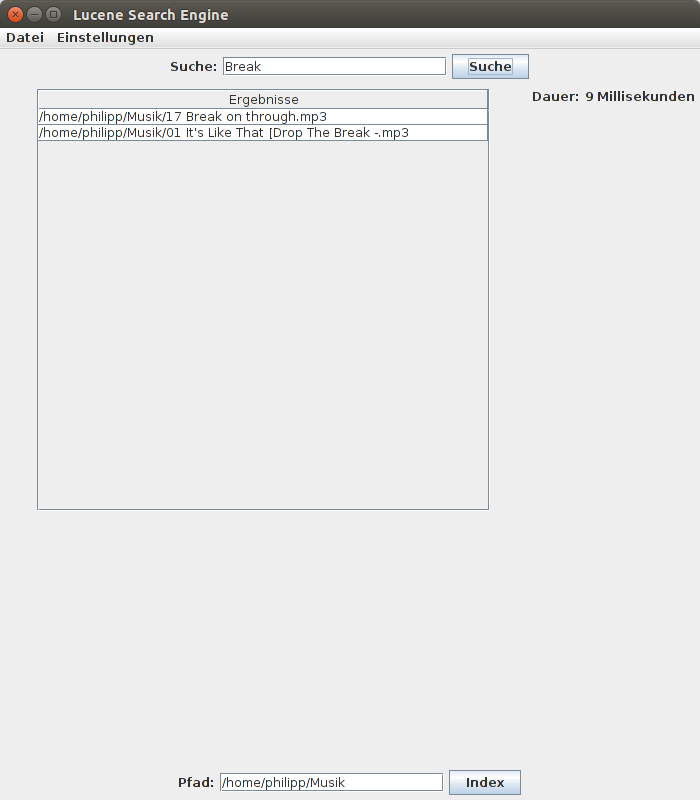
\includegraphics[width=7cm]{img/Lucene_Search_Engine_2.png}
\caption{Beispiel gesuchter Begriff\protect\footnotemark}
\end{figure}
\footnotetext{Quelle: Screenshot}
\subsection*{Der Indexer}
In diesem Teil möchte ich kurz auf die Klasse Index eingehen, welche nach den MP3-Dateien sucht und die Informationen aus den ID3-Tags zieht. Die Klasse Index wird durch das GUI gestartet, indem man den Kopf \textquotedblleft Index\textquotedblright betätigt. Als Parameter erhält er den Inhalt des Textfeldes \textquotedblleft Pfad\textquotedblright und welcher Analyzer genutzt werden soll. Nun wird der Pfad für den Index definiert. Dieser liegt immer im angegeben Verzeichnis im Unterordner \textquotedblleft Index\textquotedblright . Danach initialisiert die Klasse den Indexer und erstellt den Analyzer. Im Anschluss startet er die Messung der Zeit und beginnt die Dateien zu suchen und die Informationen zu extrahieren. Dies geschieht in der Methode index(String dataDir, FileFilter filter). Falls er einen Ordner findet, öffnet die Klasse den Ordner und sucht weiter nach Dateien.\\
\\
Hat die Methode eine MP3-Datei gefunden, wird sie mit der Methode indexFile(File f) in ein Document-Typ gewandelt, welcher die Informationen aus den ID3-Tags enthält. Per writer.addDocument(doc) wird das MP3 in den Index aufgenommen. Die ID3-Tags werden in der Methode getDocument(File f) einzeln aus jedem MP3 ausgelesen. Dabei standen verschiedene Lösungen zur Verfügung. Dazu aber später mehr im Kapitel \textquotedblleft ID3-Tags\textquotedblright .\\
\\
Sobald alle MP3-Dateien aufgenommen wurde, berechnet die Klasse als Letztes, wie lange der Vorgang gedauert hat. Dieses Ergebnis wird dann, wie schon erwähnt, auf dem GUI ausgegeben. Der Index wurde erstellt und kann nun zur Suche genutzt werden.
\subsection*{Der Searcher}
Ein Index alleine nützt uns nichts, wenn nicht ein Searcher implementiert wird, der diesen Index auch durchsuchen kann. Dazu ist in diesem Projekt die Klasse \textquotedblleft Searcher\textquotedblright vorhanden. Wie schon beim Indexer, erhält der Aufruf per Knopfdruck auf den Button \textquotedblleft Suche\textquotedblright die Parameter Pfad, Analyzerart und die Anfrage. Der Pfad wird direkt aus dem Indexpfad gelesen. So findet das Programm den korrekten Index. Danach startet die Methode search(String indexDir, String q, String analyzerArt).\\
\\
Die Methode search öffnet den vorgegebenen Pfad um den Index zu lesen. Danach wird ein Parser erstellt, der mehrere Felder absuchen kann (MultiFieldQueryParser). Je nach Analyzerart wird eine andere Version erstellt. Dieser Parser wandelt die Benutzeranfrage (hier q) so um, dass Lucene die Anfrage versteht. Die Methode durchsucht den Index und ergibt maximal 100 Ergebnisse. Die einzelnen gefundenen Inforationen werden wieder in den Typ Document umgewandelt. Zum Schluss wird eine ArrayList mit Document zurückgegeben, welche alle Ergebnisse beinhaltet. Die Liste wird jedesmal bei der Suche gelöscht und wieder von neuem befüllt. Der Inhalt der ArrayList wird zum Schluss im GUI ausgegeben, sowie auch die Dauer der Suche.
\subsection*{ID3-Tags}
ID3-Tags sind Informationen, welche direkt in die Dateien eingebettet wurden. Sie beinhalten wertvolle Informationen wie Titel, Künstler, Album, Jahr, Genre, usw. ID3 hat sich mittlerweile zum Standard für MP3 entwickelt und wird von Programmen wie iTunes, Windows Media Player und VLC genutzt. Leider können nicht alle Programme mit jeder ID3-Version umgehen. Dies kann zu Komplikationen führen.\\
\\
Um in meiner Applikation diese Daten zu extrahieren, standen drei Möglichkeiten zur Auswahl. Diese waren manuelles extrahieren in Java, benutzen einer Bibliothek und einsetzen von Tika.
\subsubsection*{Manuelles extrahieren}
Das auslesen von ID3v1 ist relativ einfach. Die Informationen sind immer fest in einem Block von 128 Bytes am Ende der Datei gespeichert. Bei Offset 3 mit einer Länge von 30 wird zum Beispiel der Songtitel gespeichert. Folgende Tabelle gibt die Felder und deren Position wieder:\\
\begin{tabular}{|c|c|l|} \hline
 \textbf{Offset} & \textbf{Länge in Bytes} & \textbf{Bedeutung}\\
 \hline
 0 & 3 & Kennung eines ID3v1-Blocks\\ \hline
 3 & 30 & Songtitel\\ \hline
 33 & 30 & Künstler\\ \hline
 63 & 30 & Album\\ \hline
 93 & 4 & Jahr\\ \hline
 97 & 30 & Kommentar\\ \hline
 127 & 1 & Genres\\ \hline
\end{tabular} \\ \\
Diese können so direkt angesprochen werden. Schwieriger wird es mit der Version 2. Ab Version zwei wird im Header der Datei angegeben, ob es sich um ID3 der Version 2 handelt. Die Tags werden dann so kodiert, dass ein Player sie nicht versteht und als fehlerhafte Informationen interpretiert. So werden die Teile der Datei übersprungen und nicht abgespielt. Neu können auch Bilder in diese Feldern abgelegt werden. Allerdings ist die Implementation sehr mühsam.
\\
\\
Da diese Lösung viel Zeit verschlingen würde, da für jede Version der ID3-Tags auch eine Methode geschrieben werden müsste, die die entsprechenden Tags ausliest, habe ich diese Lösung nicht in Betracht gezogen. Ausserdem muss ich das Rad nicht neu erfinden, wenn schon Möglichkeiten vorhanden sind, welche meine Anforderungen erfüllen. So kommen wir zum nächsten Kapitel.
\subsubsection*{Tika}
Tika ist ein Framework, das im Oktober 2008 zur Lucene-Familie hinzugefügt wurde. Es besitzt die gleichen Standard-APIs wie Lucene. Tika selber ist nur eine Ergänzung, welche verschiedene Parser für Dateien beinhaltet. Darunter auch MP3. Allerdings können laut Buch \textquotedblleft Lucene in Action\textquotedblright nur ID3v1-Tags ausgelesen werden. Dies erschwert unser vorhaben wieder, da verschiedene Versionen eingesetzt werden können. Ausserdem muss Tika auf andere Open-Source Projekte aufsetzen, um Dateien zu suchen und zu öffnen. Dies kann das Framework nicht selbst tätigen.\\
\\
Aus diesen Gründen konnte ich Tika aus meinen Möglichkeiten streichen, da so der Aufbau der Applikation nur komplizierter wurde. Und mit der Einschränkung auf ID3v1 war Tika nicht wirklich eine gute Wahl für mein Vorhaben. Ausserdem exportiert Tika die Informationen in eine XHTML-Datei. Das heisst, dass ich zusätzlich zum Index nochmals Dateien ablegen müsste. Somit blieb mir die letzte Lösung.
\subsubsection*{Extraktion mit Library}
Im Internet gibt es verschiedene Bibliotheken, die frei zur Verfügung stehen und sich um solche Dinge, wie die Extraktion von ID3-Tags, kümmern. Meine Wahl fiel auf die Lösung JAudioTagger. Dies ist ein kleines JAR-File, welches problemlos in das Projekt integriert werden konnte. Mit wenigen Code-Zeilen ermöglichte mir die Klasse, dass die Informationen aus den MP3-Dateien in den Index geschrieben werden konnten.
\\
\\
Mit 3 Zeilen wird der Vorgang initialisiert. 
\begin{lstlisting}
AudioFile audioFile = AudioFileIO.read(f);
Tag tag = audioFile.getTag();
AudioHeader header = audioFile.getAudioHeader();
\end{lstlisting}
Zeile 1 liest die Datei ein und wandelt sie in den Typ AudioFile. Durch diesen Typ können nun mit der Methode getTag() in Zeile 2 die ID3-Tags ausgelesen werden. Als Zusatz (aber hier nicht notwendig) wird der Header für weitere Funktionen aus dem AudioFile ausgelesen. Um nun die bestimmten Tags zu bekommen braucht es nur noch den folgenden Befehl:
\begin{lstlisting}
tag.getFirst(FieldKey.TITLE)
\end{lstlisting}
Mit diesem Befehl wird der spezifische Eintrag bei Titel gelesen. Diese kann dann direkt beim Indexer in ein Feld für den Typ Document gespeichert werden. Natürlich kann anstatt TITLE auch ALBUM, YEAR, ARTIST, usw. genutzt werden. Somit habe ich alle relevanten Informationen aus den Dateien extrahiert und in meinen Index geschrieben.
\newpage
\section*{Analyse der Leistung}
Die Suchleistung der Engine möchte ich über zwei Werte vergleichen. Einerseits wäre das natürlich die Zeit, welche benötigt wird, um zu indexieren und zu suchen. Andererseits muss auch das Ergebnis überprüft werden, ob auch die erwarteten Resultate zurückgegeben werden. Die Algorithmen welche verwendet werden, sind bei Lucene die Analyzer. Daher werde ich die vier gezeigten Analyzer überprüfen und danach die Werte vergleichen und ein Fazit ziehen.
\subsection*{Vorbereitung}
Um eine korrekte Messung zu bekommen, müssen für alle Analyzer die gleichen Umstände herrschen. Das heisst, dass auf einem USB-Stick eine Auswahl an Dateien gespeichert sind. Diese werden indexiert (ergibt ersten Wert). Dann wird dieser Index (der danach ebenfalls auf dem USB-Stick liegt) wird mit bestimmtem Suchabfragen gefüttert, um dann die Ergebnisse und die benötigte Zeit zu bekommen. Die Tests werden unter Windows 8.1 durchgeführt, auf einem Notebook mit einer 256GB Solid State Disk. Der USB-Stick besitzt 8GB Speicherplatz und ist von der Marke disk2go.com\\
\subsubsection*{Testmenge}
Für den Test wurden drei Ordner aus der Musikbibliothek ausgewählt. Insgesamt enthält der USB-Stick 960 Dateien und 55 Ordner. Dabei wurden Bilddateien oder ähnliche nicht entfernt. Für die Gegenüberstellung der Suchergebnisse wird das Programm MediaMonkey auf dem Computer installiert und mit der Testmenge gefüttert. Im optimalsten Fall müsste die Search Engine die gleichen Ergebnisse liefern wie das spezifizierte Suchprogramm. MediaMonkey wird in der Version 4.1.1 eingesetzt. Laut MediaMonkey sind auf dem USB-Stick 29 Genres, 257 Interpreten und 51 Alben vorhanden.
\subsection*{Zeitmessung}
In diesem Abschnitt möchte ich mich ausschliesslich um die Zeitmessungen bei den verschiedenen Analyzern kümmern. Als erstes beginnen wir mit der Messung der Indexierung. Danach kommt die Messung der Suchanfragen.
\subsubsection*{Standard Analyzer}
Wir beginnen mit dem Standard Analyzer. Zuerst möchte ich erklären, wie dieser bei der Indexierung vorgeht. Man kann den Standard Analyzer nur als umfassend einsetzbar bezeichnen. Er enthält JFlex basierten Grammatik. Somit kann er alphanummerische Werte, Akronyme, Email-Adressen, Webseiten, IP-Adresse, usw. erkennen. Ausserdem besitzt er die Stopp-Wörter, die auch der Stop-Analyzer verwendet. Bei Stop-Wörtern werden uninteressante Wörter wie Der, Die, Das ausgeblendet und nicht in die Indexierung aufgenommen. Ausserdem ist er der einzige Analyzer, der Strings wie X\&Y oder xy@zhaw.ch direkt in den Index übernimmt.\\
\\
Nun indexieren wir mit dem Standard Analyzer die Dateien auf dem USB-Stick:
\begin{figure}[h!]
\centering
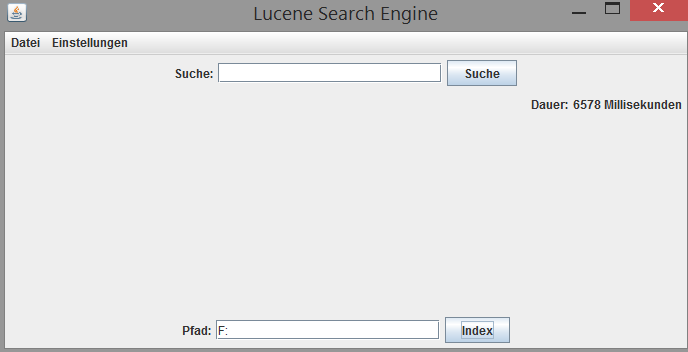
\includegraphics[width=10cm]{img/standard-analyzer-index.png}
\caption{Indexierung abgeschlossen\protect\footnotemark}
\end{figure}
\footnotetext{Quelle: Screenshot}
Wie wir auf dem Screenshot sehen brauchte die Indexierung 6578 Millisekunden um den Ordner und den Index auf dem USB-Stick zu erstellen und die Dateien zu durchforsten. Umgerechnet sind das ungefähr 6,6 Sekunden.
\subsubsection*{Simple Analyzer}
Der Simple Analyzer arbeitet auf eine sehr rudimentären Basis. Da Text bei den Analyzern immer in Tokens umgewandelt (also geteilt) werden muss, gehen die Algorithmen auf verschiedene Arten vor. Der Simple Analyzer überprüft den Text nur auf Zeichen die keine Buchstaben sind. Sobald er ein solches Zeichen gefunden hat, teilt er den String an dieser Stelle. Aus dem Beispiel des Standard Analyzers, folgt also das X\&Z zu X und Z werden würden und xy@zhaw.ch würde zu xy, zhaw und ch werden. Der Analyzer ist sehr einfach aufgebaut, müsste aber nach meiner Erwartung dafür schneller sein als der Standard Analyzer. Nach meiner Überlegung müsste nur der Whitespace Analyzer noch schneller sein. Später aber mehr dazu.
\newpage
Der Index-Ordner wird auf dem USB-Stick wieder gelöscht und erneut erstellt mit dem Simple Analyzer:
\begin{figure}[h!]
\centering
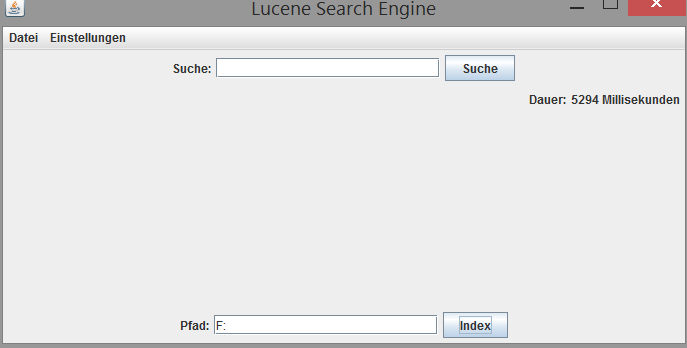
\includegraphics[width=10cm]{img/simple-analyzer-index.png}
\caption{Indexierung abgeschlossen\protect\footnotemark}
\end{figure}
\footnotetext{Quelle: Screenshot}
\\
Auch hier können wir dem Screenshot wieder ablesen, dass die Indexierung insgesamt 5294 Millisekunden gedauert hat. Die Arbeiten, die das Programm machen musste, waren die Gleichen wie schon beim Standard Analyzer. In Sekdunden umgerechnet dauerte das indexieren als ungefähr 5,3 Sekunden. Wie erwartet war dieser Analyzer schneller als der vorherige.
\subsubsection*{Whitespace Analyzer}
Wie der Simple Analyzer ist der Whitespace Analyzer sehr einfach aufgebaut. Der Text wird in diesem Fall nicht einfach nach Nicht-Buchstaben durchsucht, sondern die Tokens werden aus den Leerschlägen (Whitespaces) im Text erstellt. Wieder am Beispiel von X\&Z xy@zawh.ch würde er X\&Y und xy@zhaw.ch erkennen. Allerdings hat er, wie der Simple Analyzer das Problem, dass keine Stop-Wörter erkennt werden. Das heisst, unwichtige Wörter wie \textquotedblleft und\textquotedblright werden ebenfalls in den Index aufgenommen. Da diese Füllwörter sehr häufig vorkommen, könnten sie im Index eine höhere Gewichtung erhalten, ohne dass sie wirklich Informationen über den Text oder die Datei liefern.
\newpage
Es werden wieder die gleichen Schritte durchgeführt wie zuvor:
\begin{figure}[h!]
\centering
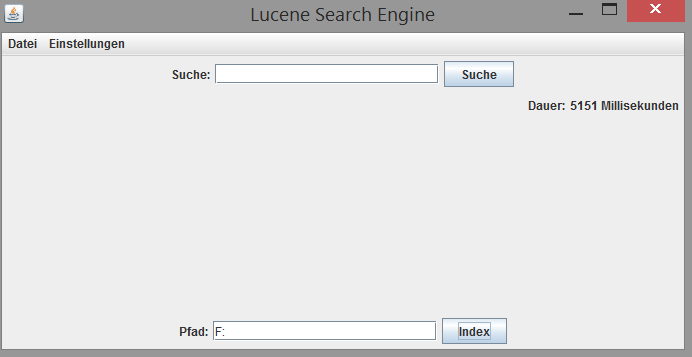
\includegraphics[width=10cm]{img/whitespace-analyzer-index.png}
\caption{Indexierung abgeschlossen\protect\footnotemark}
\end{figure}
\footnotetext{Quelle: Screenshot}
\\
Dieses Mal hat der Indexierungsvorgang 5151 Millisekunden gedauert. Wie erwartet war der Whitespace Analyzer noch ein bisschen schneller als der Simple Analyzer. Ich schätze, dass dies aus der Limitierung auf Leerzeichen kommt, da er nicht nach verschiedenen Zeichen suchen muss. Sprich für jedes Zeichen im Text muss nur eine einzige Abfrage gemacht werden. Umgerechnet sind dies ungefähr 5,2 Sekunden.
\subsubsection*{Stop Analyzer}
Der Stop Analyzer hat die Besonderheit, dass er unwichtige Wörter im Text erkennt und automatisch nicht in den Index aufnimmt. Diese Stop-Wörter können mit Listen erweitert werden, was aber in dieser Arbeit weggelassen wurde. So beschränkt sich der Stop Analyzer auf Wörter wie \textquotedblleft The\textquotedblright oder \textquotedblleft and\textquotedblright . Da die meisten MP3 auf Englisch sind, sowie deren Songtexte, ist die Standardimplementierung keine schlecht Wahl.
\newpage
Ein letztes Mal wird der Index gelöscht und die Zeit nochmals gemessen:
\begin{figure}[h!]
\centering
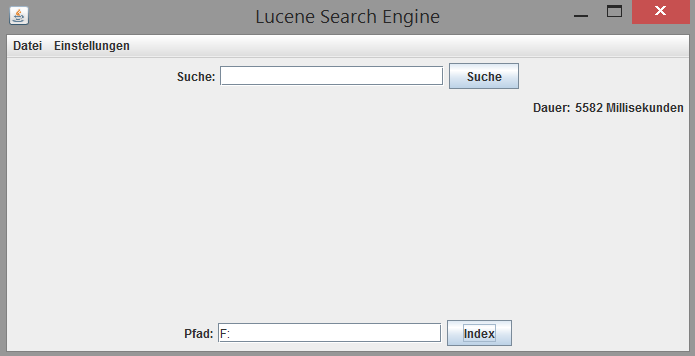
\includegraphics[width=10cm]{img/stop-analyzer-index.png}
\caption{Indexierung abgeschlossen\protect\footnotemark}
\end{figure}
\footnotetext{Quelle: Screenshot}
\\
Beim letzten Test ging die Indexierung 5582 Millisekunden. Im Vergleich zum Simple und Whitespace Analyzer hat sich die Dauer wieder erhöht. Umgerechnet in Sekunden sind das ungefähr 5.6 Sekdunden. Mit dieser Zeit liegt der Stop Analyzer aber immer noch unterhalb des Standard Analyzers. Ich erkläre mir das so, dass der Standard Analyzer komplexere Muster zu erkennen hat. Dadurch wird die Indexierung entsprechend länger brauchen.
\subsubsection*{Fazit Indexierungsdauer}
Im Vergleich haben wir nun gesehen, dass der Whitespace und der Simple Analyzer die schnellsten Verfahren sind. Mit 5,2 und 5,3 Sekunden liegen sie einiges weiter vorne als der Stop Analyzer und der Standard Analyzer. Da wir hier im Test mit einer kleinen Menge an Dateien arbeiten könnten wir das Ergebnis hochrechnen:\\
Gehen wir davon aus, dass nur MP3-Dateien in den Ordnern liegen. bei 960 Dateien mit der Gesamtgrösse von 4.6 GB, können wir abschätzen, dass eine MP3-Datei zirka 4.9 MB gross ist. Pro MP3-Datei hat der Analyzer in unserem Fall folgende Zeiten benötigt:
\begin{itemize}
	\item Standard Analyzer: 6.85 Millisekunden
	\item Simple Analyzer: 5.5 Millisekunden
	\item Whitespace Analyzer: 5.3 Millisekunden
	\item Stop Analyzer: 5.8 Millisekunden
\end{itemize}
Sagen wir nun, dass die durchschnittliche MP3-Sammlung einer Person an die 25 GB Speicherplatz braucht (Wert aus Erfahrung und Referenz der eigenen Sammlung). Dann folgt daraus, dass ungefähr 5224 MP3-Dateien vorhanden sind. Dadurch können wir sagen, wie lange die Indexierung bei dieser Menge brauchen würde:
\begin{itemize}
	\item Standard Analyzer: 35.8 Sekunden
	\item Simple Analyzer: 28.7 Sekunden
	\item Whitespace Analyzer: 27.7 Sekunden
	\item Stop Analyzer: 30.3 Sekunden
\end{itemize}
Wir sehen, je grösser die Sammlung wird, desto grösser wird der Unterschied in der Dauer der Indexierung. Immerhin ist der schnellste Analyzer um fasst 20\% schneller als der langsamste Analyzer (langsamer Analyzer wurde als 100\% gewertet).
\subsection*{Suchmessung}
Die Messung der Suchleistung teile ich in zwei Arten. Die eine Art kümmert sich um die Dauer der Suchanfrage, die andere konzentriert sich auf die gefundene Menge und ob diese Menge der erwarteten entspricht. Dazu brauchen wir aber noch eine kurze Vorbereitung, in der definiert wird, welche Suchanfragen überprüft werden. Die folgende Liste soll uns als Orientierung dienen:\\
\begin{tabular}{|l|p{10cm}|} \hline
\textbf{Suchanfrage} & \textbf{Ergebnis} \\ \hline
long way & Pfad zu:\newline 14-Do You Remember.mp3 \newline 04 Flyover.mp3 \newline 01 Hip Hop Bommi Bop (Tap Into Ameri).mp3 \newline 01 It's A Long Way To The Top (If Yo).mp3 \newline 01 It's A Long Way To The Top (If Yo).mp3 \newline 13 Long way from Liverpool.mp3 \newline 36 Stand up.mp3 \newline 13 Viva La Revolucion.mp3 \newline 18 Whole Wide World.mp3 \\ \hline
Break & Pfad zu: \newline 03 All for the sake of love.mp3 \newline 01 Ballbreaker.mp3 \newline 02 Blow Me Away.mp3 \newline 17 Break on through.mp3 \newline 08 Breaking The Rules.mp3 \newline 14 Disneyland.mp3 \newline 23 Do Anything You Wanna Do.mp3 \newline 14 Do You Remember.mp3 \newline 08 Hand of Blood.mp3 \newline 01 Heatseeker.mp3 \newline 10 I Faught The Law.mp3 \newline 01 It's Like That [Drop The Break -.mp3 \newline 03 Life Burns.mp3 \newline 13 Love Machine.mp3 \newline 04 Lovesong.mp3 \newline 09 More \& More.mp3 \newline 11 No Escape.mp3 \newline 05 Problem Child.mp3 \newline 05 Pushed Again.mp3 \newline 03 Super Shooter.mp3 \newline 20 The Great Escape.mp3 \newline 07 The Guns Of Brixton.mp3 \newline 25 The World.mp3 \newline 27 Top of the World.mp3 \newline 10 Two's Up.mp3 \newline 10 Wake the Dead.mp3 \newline 01 Who Let The Dogs Out.mp3 \\ \hline
\end{tabular}
\newpage
\begin{tabular}{|l|p{10cm}|} \hline
\textbf{Suchanfrage} & \textbf{Ergebnis} \\ \hline
instrumental & Pfad zu: \newline 03 All for the sake of love.mp3 \newline 06 Diary of a lover.mp3 \newline 09 Helmstedt Blues.mp3 \newline 16 Imperial March.mp3 \newline 13 Love Machine.mp3 \newline 09 More \& More.mp3 \newline 10 My Land.mp3 \newline 12 Perfect Criminal.mp3 \newline 01 Tote Hose.mp3 \newline 10 You Shook Me All Night Long.mp3 \\ \hline
Bells Album:Black & Pfad zu \newline 04 Hells Bells.mp3 \\ \hline
\textquotedblleft break on through\textquotedblright & Pfad zu: \newline 17 Break on through.mp3 \\ \hline
Bells OR Hit Album:Black & Pfad zu: \newline 01 Back In Black.mp3 \newline 02 Given The Dog A Bone.mp3 \newline 03 Have A Drink On Me.mp3 \newline 04 Hells Bells.mp3 \\ \hline
\end{tabular} \\ \\
Dies sind die Abfragen, welche ich verwenden werde, um die Engine zu testen. Ich lasse bewusst die Möglichkeit nach ähnlichen Wörtern zu suchen weg, da das Referenzprogramm dies ebenfalls nicht unterstützt.
\subsubsection{Standard Analyzer}
Wir starten mit dem Standard Analyzer. Da MediaMonkey bei Suchen wie long way die beiden Wörter mit AND verknüpft, wird die Abfrage in der Engine angepasst, so dass die Logik stimmt. Daher werden solche Anfragen zu long AND way. Die Screenshots zeigen die jeweiligen Ergebnisse. Die Dauer wird in der Bildunterschrift vermerkt:
\begin{figure}[h!]
\centering
	\begin{minipage}[b]{7cm}
	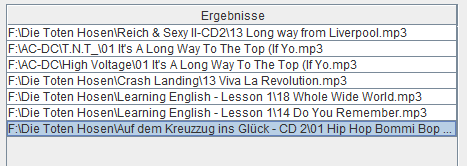
\includegraphics[width=6cm]{img/search1_stanAn_3MS.png}
	\end{minipage}
	\begin{minipage}[b]{7cm}
	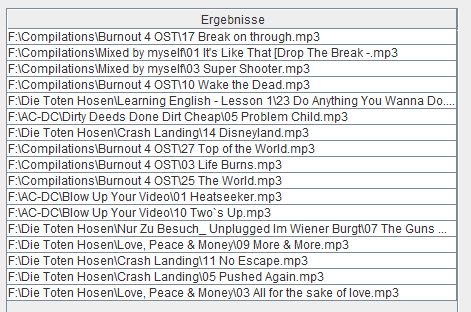
\includegraphics[width=6cm]{img/search2_stanAn_2MS.png}
	\end{minipage}
\caption{Links: Suche 1 nach 3ms, Rechts: Suche 2 nach 2ms\protect\footnotemark}
\end{figure}
\footnotetext{Quelle: Screenshot}
\begin{figure}[h!]
\centering
	\begin{minipage}[b]{7cm}
	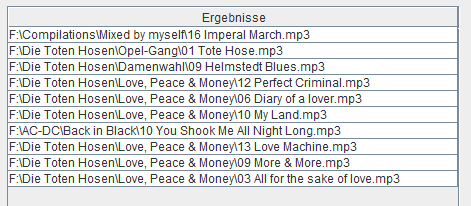
\includegraphics[width=6cm]{img/search3_stanAn_1MS.png}
	\end{minipage}
	\begin{minipage}[b]{7cm}
	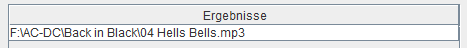
\includegraphics[width=6cm]{img/search4_stanAn_0MS.png}
	\end{minipage}
\caption{Links: Suche 3 nach 1ms, Rechts: Suche 4 nach \textless 1ms\protect\footnotemark}
\end{figure}
\footnotetext{Quelle: Screenshot}
\begin{figure}[h!]
\centering
	\begin{minipage}[b]{7cm}
	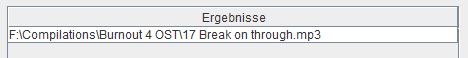
\includegraphics[width=6cm]{img/search5_stanAn_5MS.png}
	\end{minipage}
	\begin{minipage}[b]{7cm}
	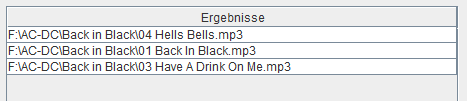
\includegraphics[width=6cm]{img/search6_stanAn_1MS.png}
	\end{minipage}
\caption{Links: Suche 5 nach 5ms, Rechts: Suche 6 nach 1ms\protect\footnotemark}
\end{figure}
\footnotetext{Quelle: Screenshot}
\subsubsection*{Simple Analyzer}
Nun wiederholen wir die Probe mit dem Simple Analyzer:
\begin{figure}[h!]
\centering
	\begin{minipage}[b]{7cm}
	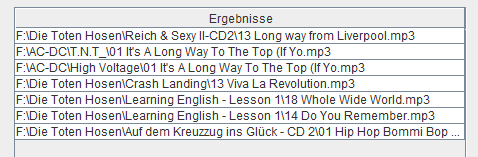
\includegraphics[width=6cm]{img/search1_simAn_28.png}
	\end{minipage}
	\begin{minipage}[b]{7cm}
	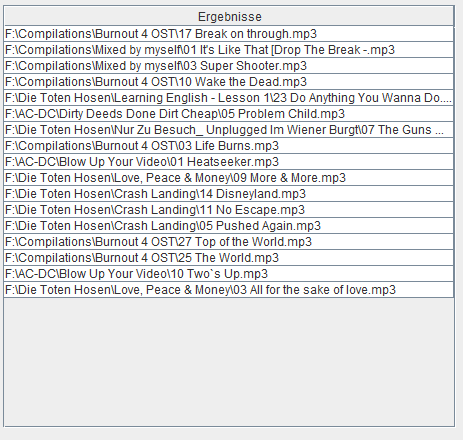
\includegraphics[width=6cm]{img/search2_simAn_0.png}
	\end{minipage}
\caption{Links: Suche 1 nach 28ms, Rechts: Suche 2 nach \textless 1ms\protect\footnotemark}
\end{figure}
\footnotetext{Quelle: Screenshot}
\begin{figure}[h!]
\centering
	\begin{minipage}[b]{7cm}
	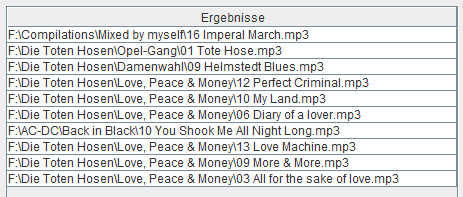
\includegraphics[width=6cm]{img/search3_simAn_4.png}
	\end{minipage}
	\begin{minipage}[b]{7cm}
	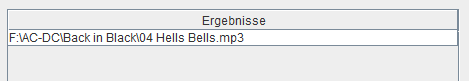
\includegraphics[width=6cm]{img/search4_simAn_0.png}
	\end{minipage}
\caption{Links: Suche 3 nach 4ms, Rechts: Suche 4 nach \textless 1ms\protect\footnotemark}
\end{figure}
\footnotetext{Quelle: Screenshot}
\begin{figure}[h!]
\centering
	\begin{minipage}[b]{7cm}
	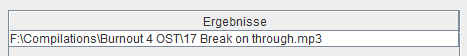
\includegraphics[width=6cm]{img/search5_simAn_15.png}
	\end{minipage}
	\begin{minipage}[b]{7cm}
	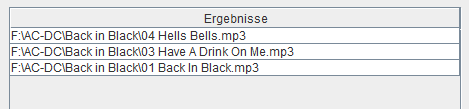
\includegraphics[width=6cm]{img/search6_simAn_0.png}
	\end{minipage}
\caption{Links: Suche 5 nach 15ms, Rechts: Suche 6 nach \textless 1ms\protect\footnotemark}
\end{figure}
\footnotetext{Quelle: Screenshot} \newpage
\subsubsection{Whitespace Analyzer}
Dieses Prozedere wiederholen wir nun nochmals für den Whitespace Analyzer:
\begin{figure}[h!]
\centering
	\begin{minipage}[b]{7cm}
	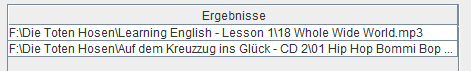
\includegraphics[width=6cm]{img/search1_whiAn_4.PNG}
	\end{minipage}
	\begin{minipage}[b]{7cm}
	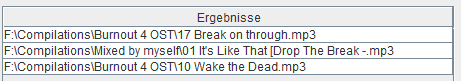
\includegraphics[width=6cm]{img/search2_whiAn_16.PNG}
	\end{minipage}
\caption{Links: Suche 1 nach 4ms, Rechts: Suche 2 nach 16ms\protect\footnotemark}
\end{figure}
\footnotetext{Quelle: Screenshot}
\begin{figure}[h!]
\centering
	\begin{minipage}[b]{7cm}
	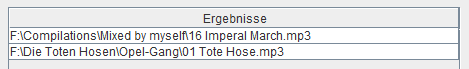
\includegraphics[width=6cm]{img/search3_whiAn_4.PNG}
	\end{minipage}
	\begin{minipage}[b]{7cm}
	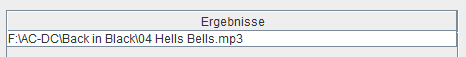
\includegraphics[width=6cm]{img/search4_whiAn_16.PNG}
	\end{minipage}
\caption{Links: Suche 3 nach 4ms, Rechts: Suche 4 nach 16ms\protect\footnotemark}
\end{figure}
\footnotetext{Quelle: Screenshot}
\begin{figure}[h!]
\centering
	\begin{minipage}[b]{7cm}
	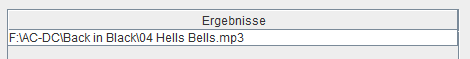
\includegraphics[width=6cm]{img/search6_whiAn_15.PNG}
	\caption{Suche 6 nach 15ms\protect\footnotemark}
	\end{minipage}
\end{figure}
\footnotetext{Quelle: Screenshot}
\newpage
\subsubsection*{Stop Analyzer}
Ein letztes Mal führen wir nun die Analyse durch:
\begin{figure}[h!]
\centering
	\begin{minipage}[b]{7cm}
	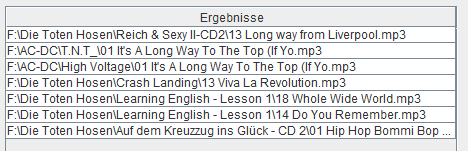
\includegraphics[width=6cm]{img/search1_stoAn_16.PNG}
	\end{minipage}
	\begin{minipage}[b]{7cm}
	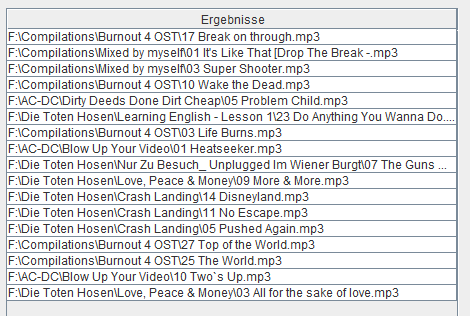
\includegraphics[width=6cm]{img/search2_stoAn_0.PNG}
	\end{minipage}
\caption{Links: Suche 1 nach 16ms, Rechts: Suche 2 nach \textless 1ms\protect\footnotemark}
\end{figure}
\footnotetext{Quelle: Screenshot}
\begin{figure}[h!]
\centering
	\begin{minipage}[b]{7cm}
	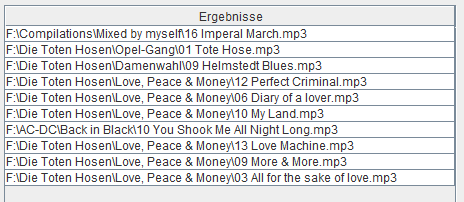
\includegraphics[width=6cm]{img/search3_stoAn_16.PNG}
	\end{minipage}
	\begin{minipage}[b]{7cm}
	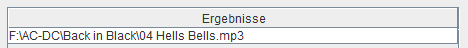
\includegraphics[width=6cm]{img/search4_stoAn_0.PNG}
	\end{minipage}
\caption{Links: Suche 3 nach 16ms, Rechts: Suche 4 nach \textless 1ms\protect\footnotemark}
\end{figure}
\footnotetext{Quelle: Screenshot}
\begin{figure}[h!]
\centering
	\begin{minipage}[b]{7cm}
	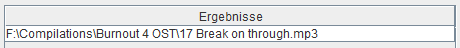
\includegraphics[width=6cm]{img/search5_stoAn_16.PNG}
	\end{minipage}
	\begin{minipage}[b]{7cm}
	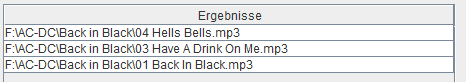
\includegraphics[width=6cm]{img/search6_stoAn_15.PNG}
	\end{minipage}
\caption{Links: Suche 5 nach 16ms, Rechts: Suche 6 nach 15ms\protect\footnotemark}
\end{figure}
\footnotetext{Quelle: Screenshot}
\newpage
\subsubsection*{Auswertung und Fazit}
Vergleichen wir nun die verschiedenen Werte der Suche, kommen wir auf folgendes Ergebnis: \\
\begin{tabular}{|l|c|c|c|c|} \hline
 & \textbf{Standard} & \textbf{Simple} & \textbf{Whitespace} & \textbf{Stop} \\ \hline
Hits Suche 1 & 7/9 & 7/9 & 2/9 & 7/9\\
Hits Suche 2 & 17/27 & 17/29 & 3/29 & 17/29\\
Hits Suche 3 & 10/10 & 10/10 & 2/10 & 10/10\\
Hits Suche 4 & 1/1 & 1/1 & 1/1 & 1/1\\
Hits Suche 5 & 1/1 & 1/1 & 0/1 & 1/1\\
Hits Suche 6 & 3/4 & 3/4& 1/4 & 3/4\\ \hline
Dauer Suche 1 & 3 & 28 & 4 & 16\\
Dauer Suche 2 & 2 & \textless 1 & 16 & \textless 1\\
Dauer Suche 3 & 1 & 4 & 4 & 16\\
Dauer Suche 4 & \textless 1 & 1 & 16 & \textless 1\\
Dauer Suche 5 & 5 & 15 & - & 16\\
Dauer Suche 6 & 1 & \textless 1 & 15 & 15\\ \hline
\end{tabular} \\ \\
Wir erkennen also, dass kein Analyzer alle Einträge gefunden hat. Besonders bei Suche 2 gehen viele verloren. Zu erwähnen ist der Whitespace Analyzer, da dieser beim Indexieren zwar sehr schnell war, hingegen bei der Suchleistung und der benötigten Zeit sehr schwach ist. So hat er bei Suche 5 kein Resultat geliefert. Obwohl der Standard Analyzer lange indexiert, ist dafür seine Suchleistung sehr gut. Er hat den grossen Teil der Dateien gefunden und das in einer sehr guten Zeit.\\
\\
Schlussendlich muss man sagen, dass es wohl nicht den einen Analyzer gibt, welche alle Fälle sehr gut abdeckt. Steht der Fokus auf einer schnellen Indexierung, ist der Whitespace Analyzer wohl die erste Wahl. Hingegen bei einer optimalen Suchleistung würde ich in diesem Fall zum Standard Analyzer raten.
\end{document}